% default fontsize is 10pt
\documentclass[11pt,a4paper]{article}
\usepackage{packages}

\addbibresource{references.bib}

% Set the title for table of contents
\newcommand{\ContentsName}{Table of Contents}
\addto\captionsenglish{\renewcommand*\contentsname{\ContentsName}}

\makeglossaries
\loadglsentries{glossaries}

\newcommand{\TocSpacing}{0em}
\newcommand{\ParagraphSpacing}{0.8em}
\newcommand{\ParagraphIndentation}{0pt}
\newcommand{\LineSpacing}{1}

\setlength\parindent{\ParagraphIndentation}
\renewcommand\baselinestretch{\LineSpacing}

\begin{document}
    \nocite{*}

    \begin{titlepage}
        \centering
        ~\\
        \vspace{1cm}
        {\mdseries Bachelorthesis \par}
        {\mdseries Computer Science\par}
        \vspace{1.5cm}
        {\huge\bfseries HybridCloudOps Models for Business Application Development\par}
        \vspace{2cm}
        {\Large Simon Anliker\par}
        ~\\
        {\Large \url{https://anliker.dev}\par}
        \vfill
        {\Large July 19, 2020\par}
    \end{titlepage}
    \clearpage

    \setlength\parskip{\ParagraphSpacing}

    \section*{Preface}
    \addcontentsline{toc}{section}{Preface}
    \subfile{preface}
    \clearpage

    \section*{Acknowledgements}
    \addcontentsline{toc}{section}{Acknowledgements}
    \subfile{acknowledgements}
    \clearpage

    \setlength\parskip{\TocSpacing}
    \phantomsection
    \addcontentsline{toc}{section}{\ContentsName}
    \tableofcontents
    \setlength\parskip{\ParagraphSpacing}
    \clearpage

    \phantomsection
    \addcontentsline{toc}{section}{Abstract}
    \subfile{abstract}
    \clearpage
    \subfile{abstract_de}
    \clearpage

    \section{Introduction}
    \label{sec:introduction}

    \subfile{intro}

    \clearpage
    \section{Definitions}
    \label{sec:definitions}

    \subfile{definitions}

    \clearpage
    \section{Concepts}
    \label{sec:concepts}

    \subfile{concepts}

    \clearpage
    \section{Methodology}
    \label{sec:methodology}

    \subfile{methodology}

    \clearpage
    \section{Instrumentation}
    \label{sec:implementation}

    \subfile{impl}

    \clearpage
    \section{Results}
    \label{sec:results}

    \subfile{results}

    \clearpage
    \section{Discussion and Outlook}
    \label{sec:outlook}

    \subfile{outlook}

    \clearpage
    \listoffigures

    \listoftables

    \listofalgorithms

    \printglossary[type=\acronymtype]

    \printglossary

    \clearpage
    \phantomsection
    \addcontentsline{toc}{section}{References}
    \printbibliography

    \clearpage
    \section*{Appendix}
    \addcontentsline{toc}{section}{\protect\numberline{A} Appendix}

    \clearpage
    \subsection*{Thesis assignment}
    \addcontentsline{toc}{subsection}{\protect\numberline{A1} Thesis assignment}
    \subfile{assignment}

    \clearpage
    \phantomsection
    \addcontentsline{toc}{subsection}{\protect\numberline{A2} Project management}
    Removed in this version.

    \clearpage
    \subsection*{User manual}
    \addcontentsline{toc}{subsection}{\protect\numberline{A3} User manual}
    \subfile{manual}

    \clearpage
    \subsection*{Assessment questionnaire}
    \addcontentsline{toc}{subsection}{\protect\numberline{A4} Assessment}
    The assessment questionnaire shows the Google Forms content that has been used during the interview with the expert group to gather feedback.
    The processed feedback is shown as part of the results data.
    The raw feedback data is handed in as part of the submission content.
    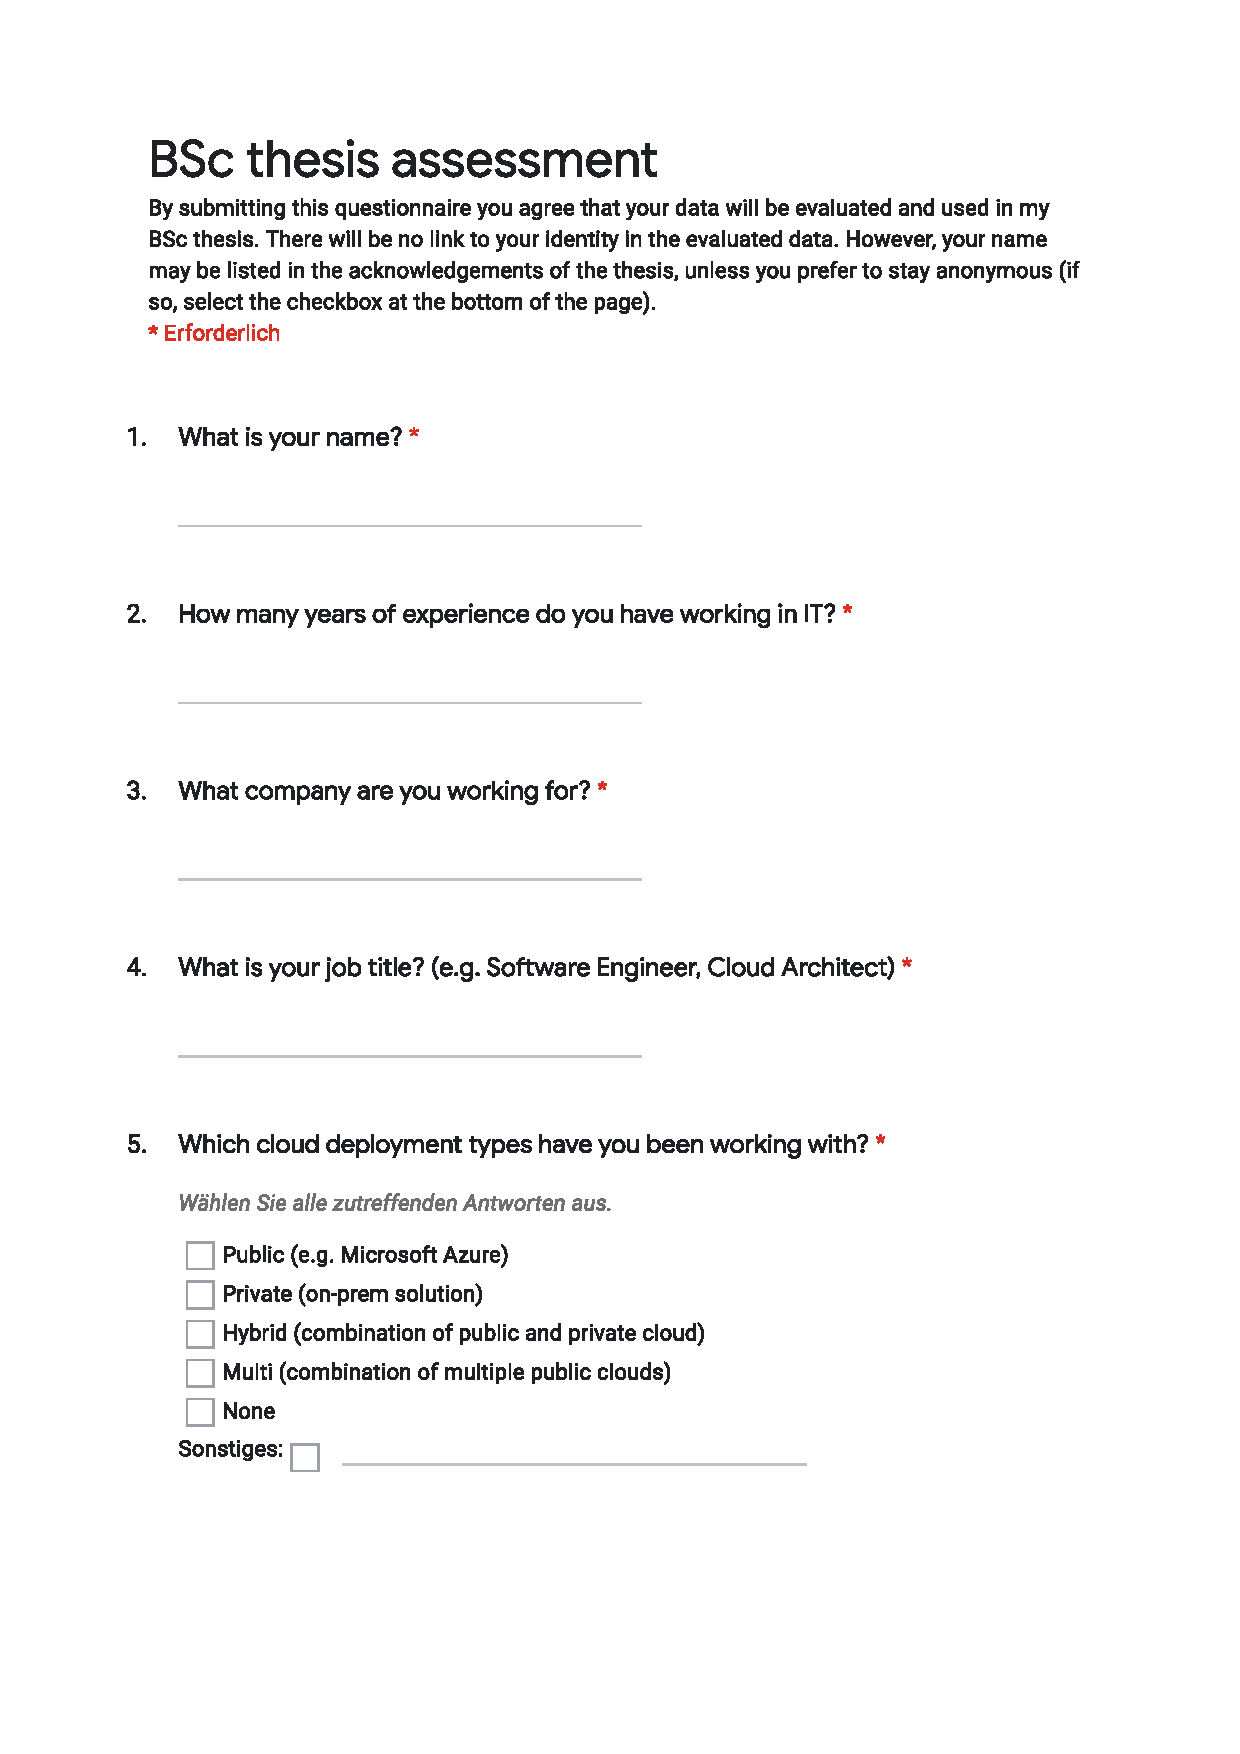
\includepdf[pages={1-}, pagecommand={}]{appendix-assessment.pdf}

    \clearpage
    \subsection*{Results data}
    \addcontentsline{toc}{subsection}{\protect\numberline{A5} Results data}
    The results data shows the processed data resulting in the diagrams and graphs used in the results section of the thesis.
    The raw data used for processing is handed in as part of the submission content.
    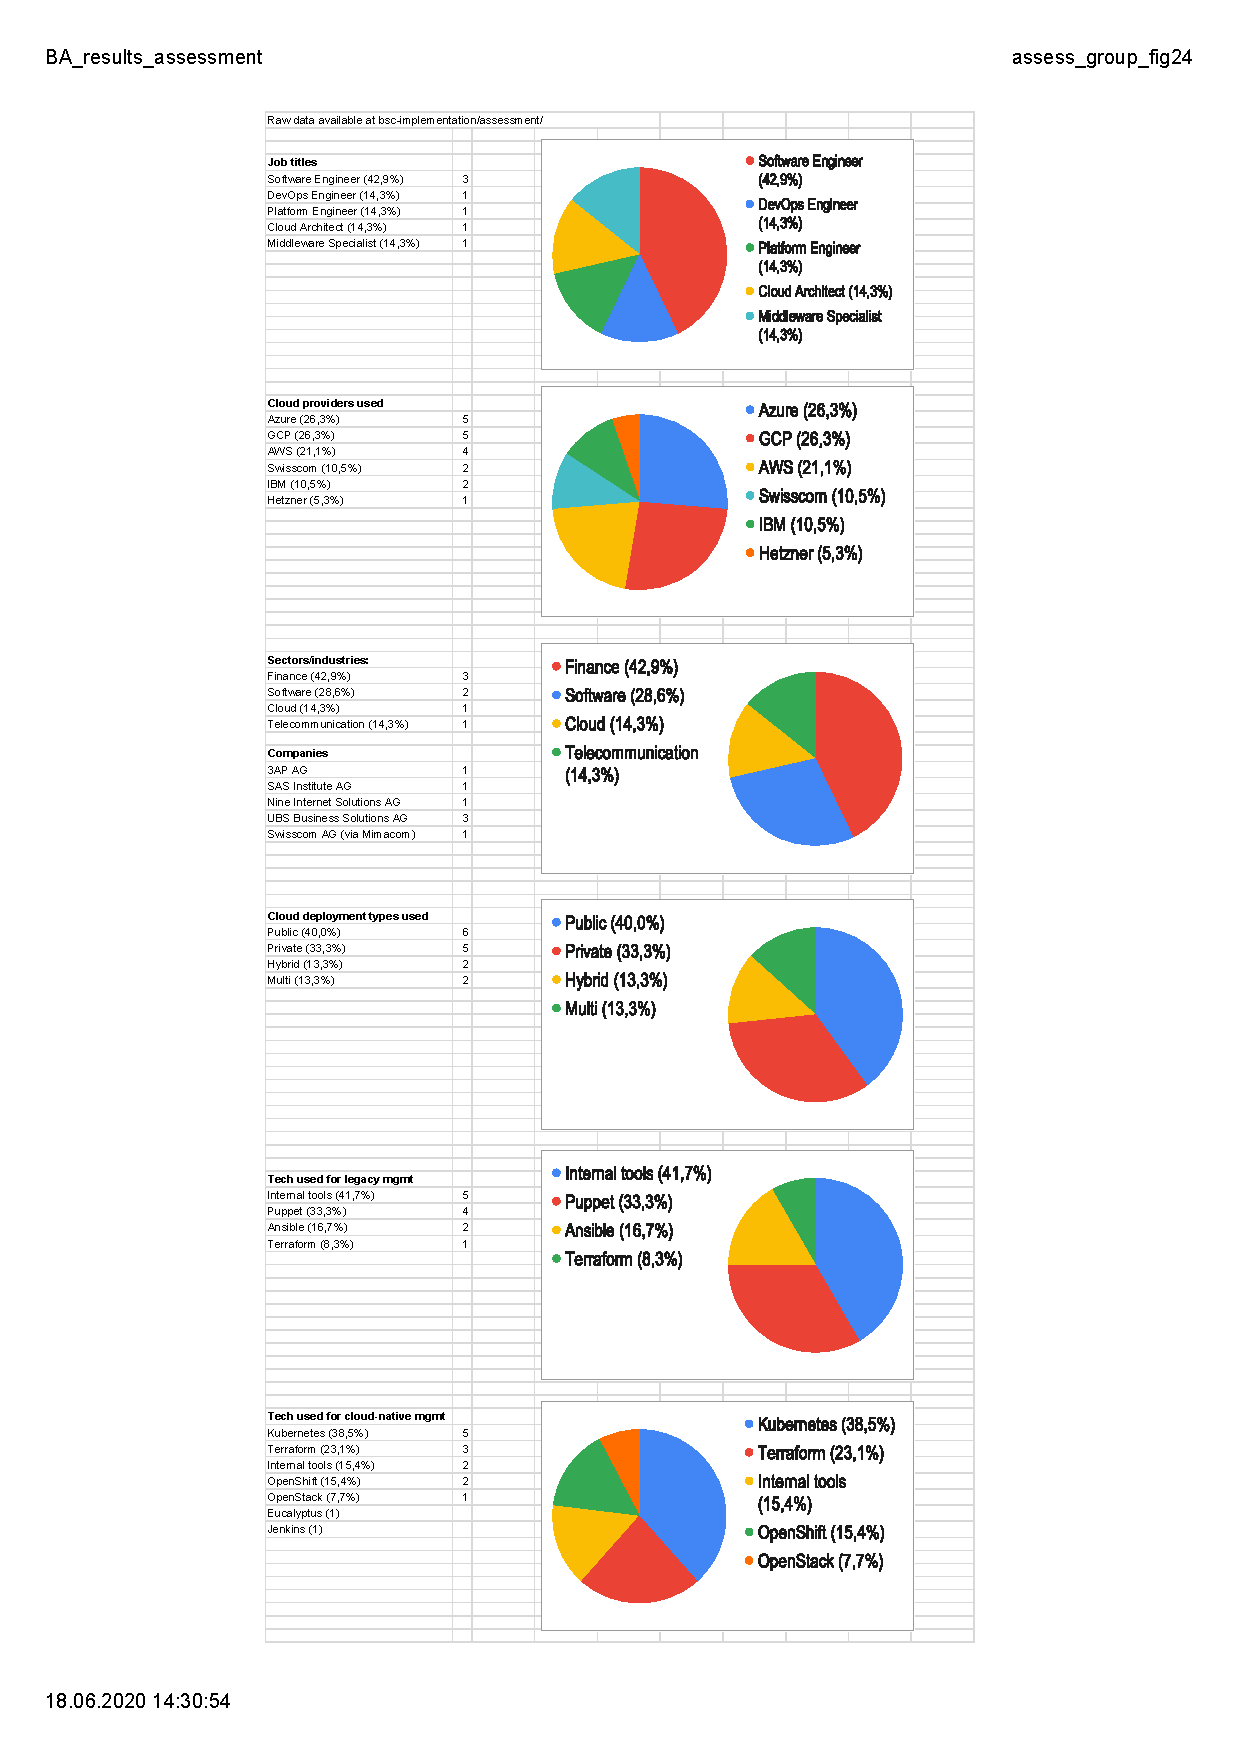
\includepdf[pages={1-}, pagecommand={}]{appendix-results-assessment.pdf}
    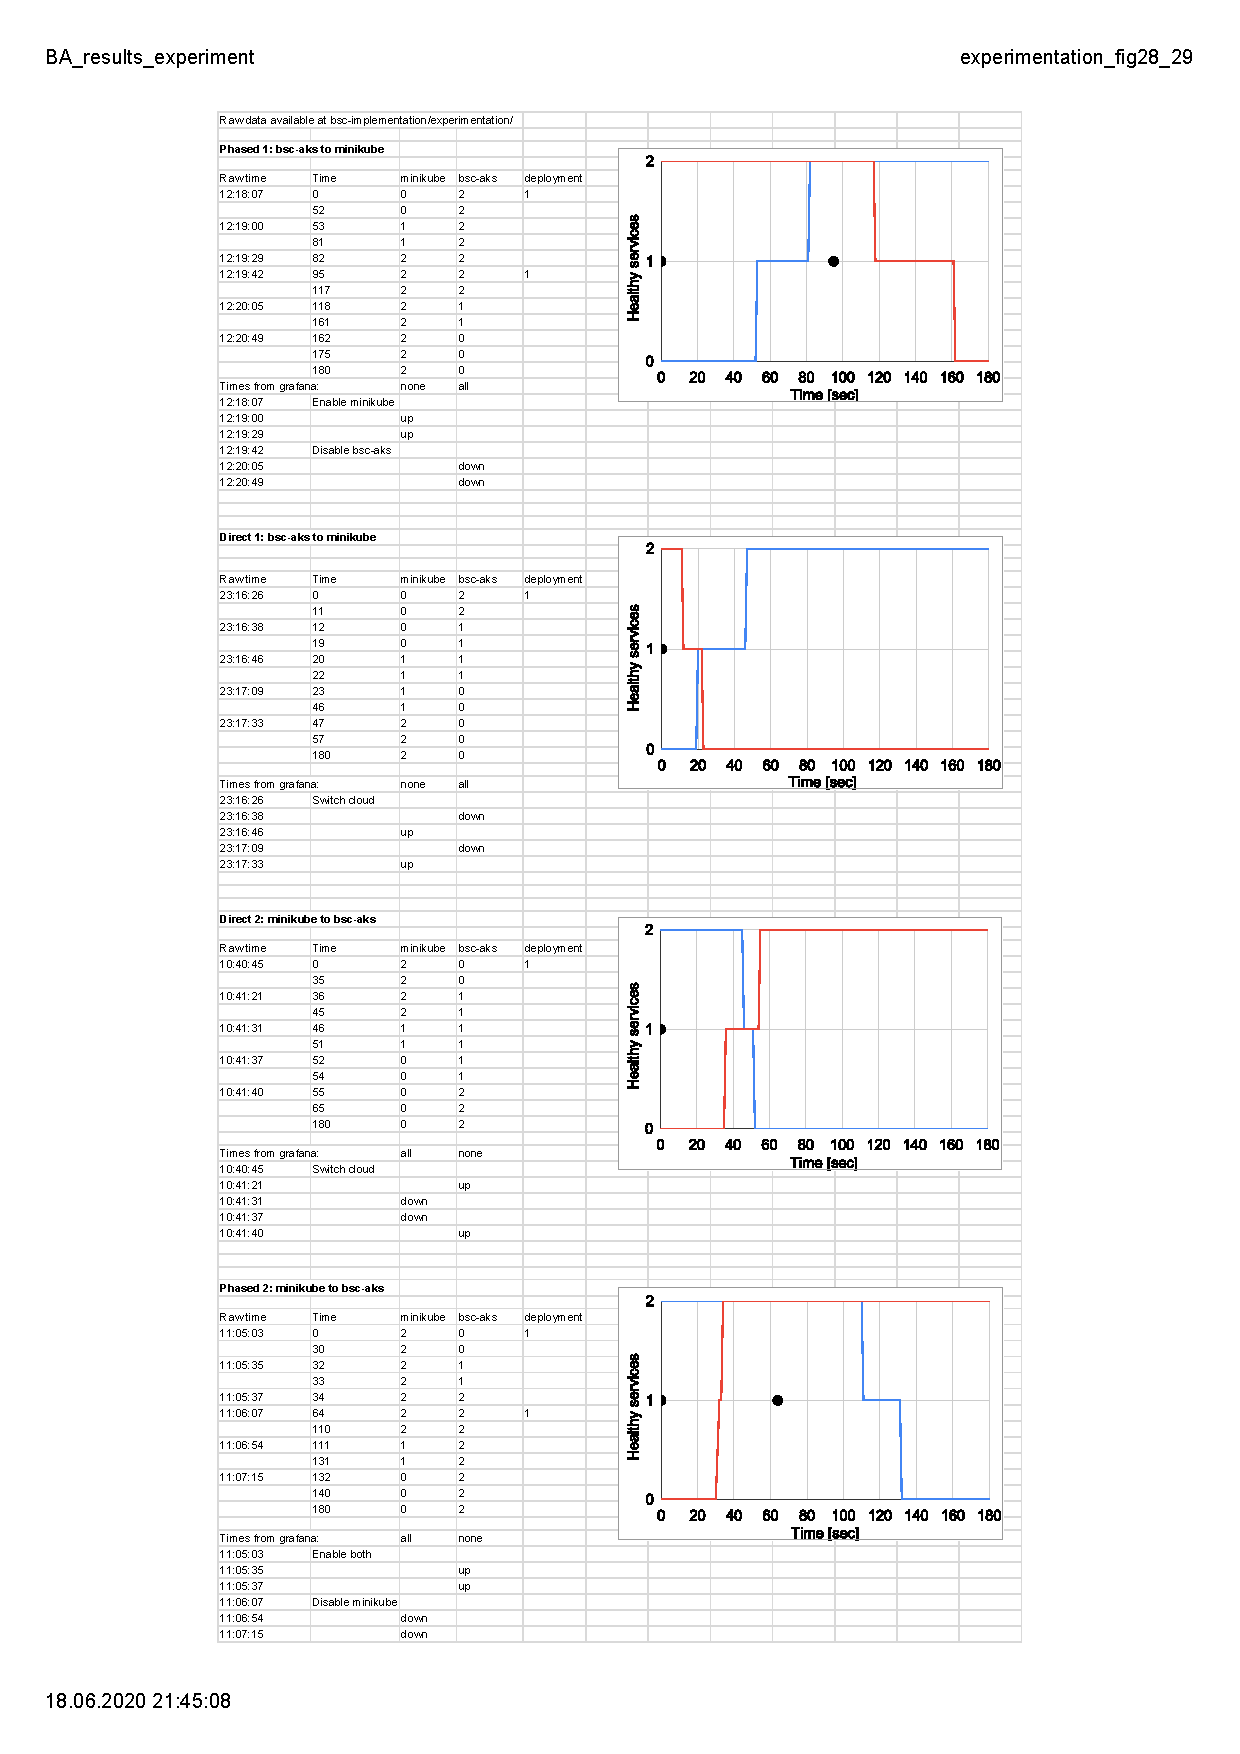
\includepdf[pages={1-}, pagecommand={}]{appendix-results-experiments.pdf}

    \clearpage
    \phantomsection
    \addcontentsline{toc}{subsection}{\protect\numberline{A6} Paper collection}
    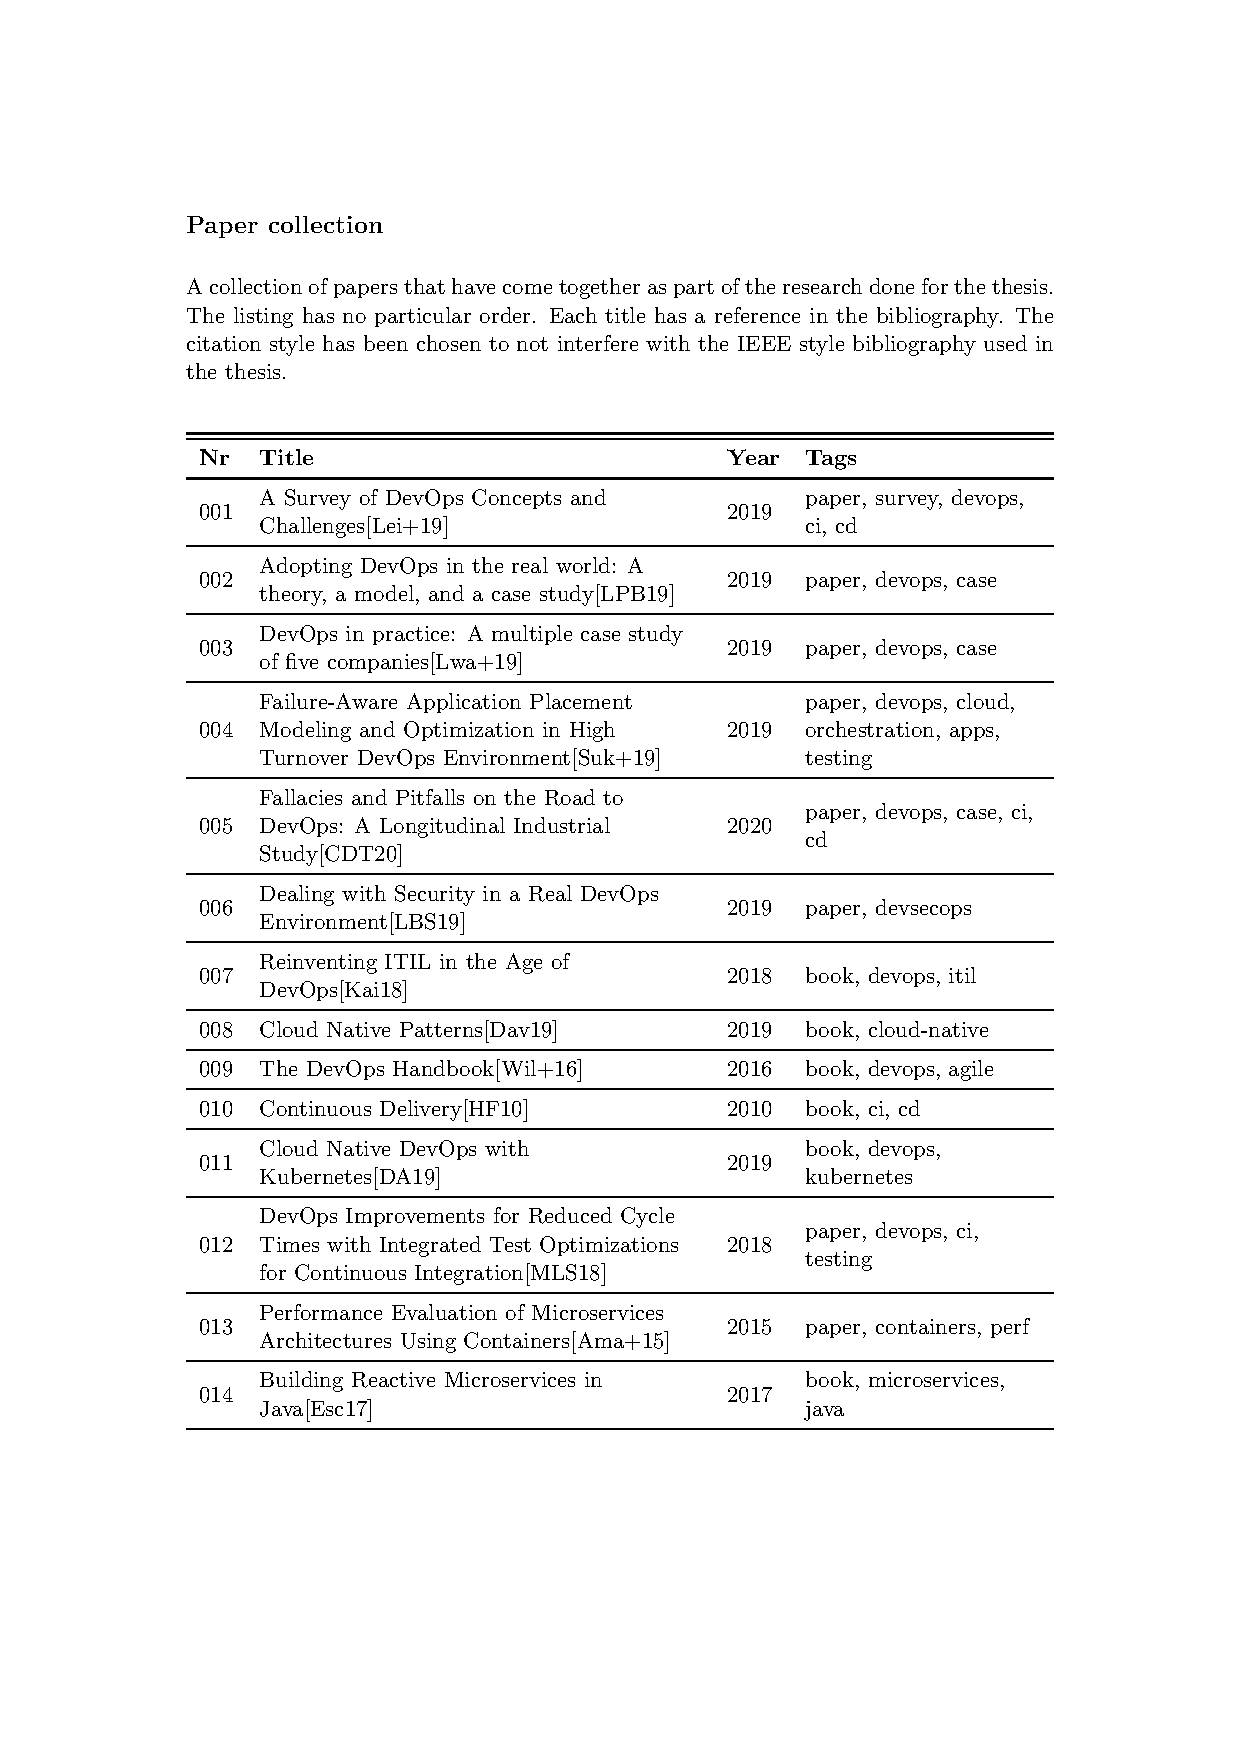
\includepdf[pages={1-}, pagecommand={}]{appendix-papers.pdf}

    \clearpage
    \subsection*{Submission content}
    \addcontentsline{toc}{subsection}{\protect\numberline{A7} Submission content}
    Removed in this version.

\end{document}








